\section{Review of Hippocampus models}
\subsection{Hippocampus biology}
The hippocampus \cite{andersen2006hippocampus}  is involved in the creation and consolidation of memories, in a circuit along with the Entorhinal Cortex (EC) and Dentate Gyrus (DG).
The main function of the hippocampus is thought to be the consolidation of associative memories and spatial memory.
As such it can be considered suitable for navigation within an environment, associating each place with sensory memories about that place.

The hippocampus is comprised of four main sub-fields: CA1, CA2, CA3 and CA4.
However, the classical view of the hippocampal circuit only considers the CA1 and CA3 sub-fields, along with the EC and DG.
The circuit accepts input from external sources and the response from the CA1 sub-field.
This is then passed to the DG which sparsifies the EC output.
The output of the EC is also passed to the CA3 sub-field along with the output of the DG.
The CA3 sub-field also accepts recurrent connections.
This allows it to consolidate interactions between old
 and new stimuli.
CA3 then projects its output to the CA1 sub-field, which provides the main output to the rest of the limbic system.
This structure is shown in \figureref{fig:hippocampus}

\picturesque{figures/lit_biology/CajalHippocampus.png}{Visual representation of the hippocampal circuit, modified from the \cite{imghippooriginal} original by \cite{imghippo}.}{fig:hippocampus}

% \begin{figure}
%     \centering
%     \includegraphics{}
%     \caption{Classical Circuit of the hippocampus}
%     \label{fig:bio_hippocampus}
% \end{figure}
%\textbf{\color{red}CF: you can mostly paraphrase this from my previous papers here. It is traditional to include some pictures of brains here. HC is supposed to look like a seahorse and there are pictures of that.}
\subsection{Hippocampal model - Unitary Coherent Particle Filter}
\label{subsubsec:ucpf}
%\textbf{\color{red}CF: you can mostly paraphrase this from my previous papers here. You can include figures showing the model structures here.}

% CF: the reader will not understand the model. You need to show a diagram of the model itself and describe its components with full mathmatical details.
The initial model of the unitary coherent particle filter of hippocampus (UCPF-HC) by \cite{foxandprescott2010A} uses handset weights to initialise the model and understand how it initially evolves. 
This is further expanded to use sensors to differentiate between locations within a simple environment.

 \picturesque{figures/lit_biology/alan_model.png}{Illustration of the hippocampus model showing data flows and hippocampus regions. SURF features are the new visual inputs. (Subiculum circuit not shown.) from \cite{saul2011}}{fig:ourcircuit}

The model is comprised of 4 main areas, an EC representation, a DG representation, the CA3 subfield and the CA1 subfield.
The EC and DG are used to provide input from the outside world to the model, encoding them into lamellae.
They project to the CA3 sub-field, which is represented in the model by a modified Temporal Restricted Boltzmann Machine(TRBM), proposed by \citep{hintonDBN2006}.
This allows the CA3 sub-field to be represented by the joint probability distribution:
\begin{equation}
    P(x_t, x_{t-1}, z_t) = \frac{1}{Z}\exp\sum_t(-x_t' W_{x_t'x_t'} x'_{t-1} - x'_tW_{x'_tz'_t}z'_t )
\end{equation}

In this distribution, $z$ represents a boolean observation vector, $x$ represents a boolean hidden state vector and the weight matrices between them.
This distribution, in conjunction with the modification of the standard Temporal Restricted Boltzmann Machine allows for a deterministic update, obtaining maximum \textit{a posteriori} estimates,

\begin{equation}
    \hat{x_t} \leftarrow arg \max   P(x_t|\hat{x_{t-1}},z_t) = \{\hat{x_t}(i)=(P(x_t(i)|\hat{x_{t-1}},z_t) > \frac{1}{2})\}_i
    \label{eqn:post}
\end{equation}

%  this does not make sense
% \wording
which is considered to be a zero temperature limit of the annealed sequential Gibbs sampler.
This sampler gives a set of boolean values, which can then be used to identify where the model believes it is in the environment. 
These boolean values can then be decoded into the CA1 sub-field, which projects back to the EC, completing the circuit.




% \note{paragraph on how different parts of the model map to the Hippocampus}
% \begin{figure}
%     \centering
%     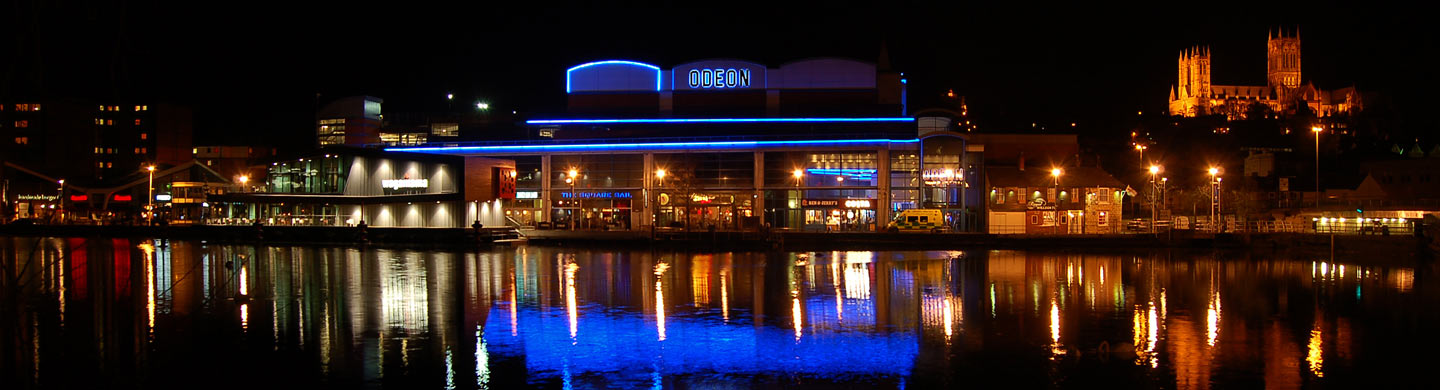
\includegraphics{figures/brayford.jpg}
%     \caption{Map of hippocampus to model.}
%     \label{fig:}
% \end{figure}